\chapter{Équations de Maxwell, covariance et ondes électromagnétiques}

\lectureoverview{Les champs électrique et magnétique agissent sur la matière chargée par l’intermédiaire de la force de Lorentz, mais la matière doit aussi créer et réorganiser les champs. Nous formulerons cette réciprocité de l’électromagnétisme, montrerons que les équations de Maxwell sont covariantes de Lorentz, en dériverons les solutions ondulatoires, puis réintroduirons la charge et le courant sous une forme qui rend manifeste la conservation locale. Dans tout ce cours, nous utilisons des unités telles que \(c=1\).}

\section{L’autre aspect de l’électromagnétisme}

Commençons par la partie du sujet déjà étudiée. Si une particule de charge \(q\) se déplace à la vitesse \(\mathbf v\) dans des champs électrique et magnétique, la force est
\begin{equation}
\mathbf F=q\bigl(\mathbf E+\mathbf v\times\mathbf B\bigr).
\label{eq:lorentz-force-three}
\end{equation}
Le facteur \(q\) est indispensable. Une particule non chargée ne subit pas la force électromagnétique. Le champ électrique contribue même lorsque la particule est momentanément au repos, tandis que la contribution magnétique dépend de son mouvement.

L’équation~\eqref{eq:lorentz-force-three} nous indique l’effet de champs prescrits sur la matière. Elle ne nous dit pas ce qui détermine les champs. Qu’est-ce qui produit un champ électrique autour d’un objet, un champ magnétique autour d’un autre, ou une onde qui se propage dans le vide ? Les équations qui répondent à ces questions sont les équations de Maxwell.

\begin{figure}[H]
\centering
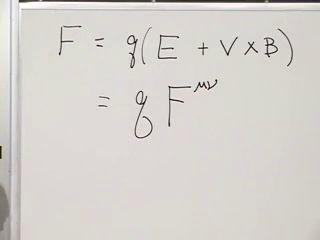
\includegraphics[width=0.62\textwidth]{lecture_58_figure_02.png}
\caption{La force de Lorentz en trois dimensions et le début de sa reformulation tensorielle.}
\lectureframe{00:05:49}
\end{figure}

La forme relativiste de la loi de force annonce les notations dont nous aurons besoin :
\begin{equation}
f^\mu=qF^\mu{}_{\nu}u^\nu.
\label{eq:lorentz-force-four}
\end{equation}
Ici, \(u^\nu\) est la quadrivitesse, \(f^\mu\) la quadri-force, et \(F^{\mu\nu}\) un tenseur antisymétrique construit à partir de \(\mathbf E\) et \(\mathbf B\). Au tableau, on n’en écrit d’abord que le début schématique ; la contraction avec \(u^\nu\) fournit le vecteur manquant et laisse un indice de force libre.

Il y a une raison physique pour laquelle la matière doit agir en retour sur le champ. Une onde électromagnétique peut frapper une charge, l’accélérer et lui transférer de l’énergie. Si le champ pouvait agir sur la charge sans que celle-ci puisse jamais agir sur le champ, il n’y aurait aucune source à laquelle retirer cette énergie. L’action et la réaction ne suffisent pas tout à fait à expliquer cela, mais la conservation de l’énergie rend inévitable ce couplage réciproque.

\section{Une source variable émet une perturbation}

Une charge ponctuelle produit un champ électrique dirigé vers l’extérieur ou vers l’intérieur à partir de sa position. Un courant dans un fil--un flux de particules chargées--produit un champ magnétique qui circule autour du fil. Ces images familières de situations statiques montrent déjà deux configurations géométriques différentes : le flux électrique émane des charges, tandis que les lignes de champ magnétique s’enroulent autour du courant.

Déplaçons maintenant brusquement la charge ponctuelle. Près de sa nouvelle position, le champ électrique doit commencer à se réorganiser, mais un observateur éloigné ne peut pas apprendre instantanément que la charge s’est déplacée. Au loin, l’ancien champ persiste jusqu’à l’arrivée du signal. Entre les régions proche et lointaine se trouve un front mobile où le champ est en train de changer. Cette réorganisation qui se propage est une perturbation électromagnétique.

Si la charge est animée d’un mouvement de va-et-vient, des réorganisations successives se suivent et forment une onde électromagnétique. C’est le fonctionnement élémentaire d’une antenne : un courant électrique oscillant émet une perturbation du champ vers l’extérieur. Inverser le sens du courant dans un fil conduit au même raisonnement pour le champ magnétique. Le sens de circulation de \(\mathbf B\) doit s’inverser, mais cette inversion se propage au lieu d’apparaître partout à la fois.

Cette image causale fixe deux objectifs aux équations de Maxwell. Elles doivent décrire comment la charge et le courant sont à l’origine des champs, et permettre aux variations de ces champs de se propager à une vitesse qui ne dépasse pas celle de la lumière. Le second objectif met aussi la relativité à l’épreuve. Si les équations de Maxwell ont la même forme dans tous les référentiels inertiels et impliquent une vitesse d’onde bien déterminée, alors elles doivent conduire chaque référentiel inertiel à déduire la même vitesse.

\section{Rappel sur l’équation d’onde relativiste}

Avant de passer aux champs vectoriels, considérons un champ scalaire \(\phi(\mathbf x,t)\), qui prend une valeur numérique en chaque point de l’espace-temps. Une équation du premier ordre,
\begin{equation}
\partial_\mu\phi=0
\end{equation}
signifierait que toutes les dérivées spatio-temporelles s’annulent. Le champ serait constant et ne pourrait donc pas porter d’onde. Une équation d’onde relativiste non triviale fait intervenir deux dérivées :
\begin{equation}
\partial_\mu\partial^\mu\phi=0.
\end{equation}
Avec la convention de signe utilisée ici,
\begin{equation}
\left(\partial_t^2-\partial_x^2-\partial_y^2-\partial_z^2\right)\phi=0,
\label{eq:scalar-wave-four}
\end{equation}
ou, sous une forme plus compacte,
\begin{equation}
\left(\partial_t^2-\nabla^2\right)\phi=0.
\end{equation}
Le choix \(c=1\) permet d’exprimer le temps et les distances dans des unités compatibles. Si l’on rétablit les unités usuelles, le facteur \(1/c^2\) apparaît devant la dérivée temporelle seconde.

Pour une onde qui se propage le long de l’axe \(z\), le champ dépend de \(z\) et de \(t\), mais ni de \(x\) ni de \(y\). L’équation~\eqref{eq:scalar-wave-four} se réduit à
\begin{equation}
\left(\partial_t^2-\partial_z^2\right)\phi=0.
\label{eq:scalar-wave-one}
\end{equation}

\begin{figure}[H]
\centering
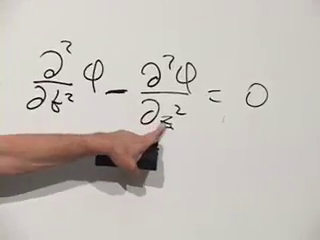
\includegraphics[width=0.56\textwidth]{lecture_58_figure_04.png}
\caption{L’équation d’onde scalaire à une dimension, modèle des ondes électromagnétiques.}
\lectureframe{00:47:03}
\end{figure}

La forme générale d’une onde progressive est
\begin{equation}
\phi(z,t)=f(z-t)+g(z+t).
\end{equation}
Le profil \(f(z-t)\) se propage dans le sens des \(z\) croissants, car un point de phase constante vérifie \(z-t=\text{constant}\). Le profil \(g(z+t)\) se propage dans le sens opposé. Rien n’impose que l’un ou l’autre profil soit sinusoïdal ; toute forme suffisamment régulière se translate sans se déformer.

Les sinusoïdes sont néanmoins commodes :
\begin{equation}
\phi(z,t)=A\cos\!\bigl(k(z-t)\bigr).
\end{equation}
Le nombre d’onde \(k\) détermine la longueur d’onde :
\begin{equation}
\lambda=\frac{2\pi}{k}.
\end{equation}
Une grande valeur de \(k\) produit des oscillations spatiales rapides et une courte longueur d’onde ; une petite valeur de \(k\) produit une longue longueur d’onde. Ces mêmes profils deviendront bientôt des composantes de \(\mathbf E\) et de \(\mathbf B\).

\section{Les outils de calcul vectoriel nécessaires aux équations de Maxwell}

Les équations de Maxwell font intervenir des produits scalaires, des produits vectoriels, la divergence et le rotationnel. Il est utile de reprendre une fois ces notations, car les calculs en composantes qui suivent reposent précisément sur ces opérations.

Pour les vecteurs usuels \(\mathbf a\) et \(\mathbf b\), le produit scalaire est le scalaire
\begin{equation}
\mathbf a\cdot\mathbf b
=a_xb_x+a_yb_y+a_zb_z.
\end{equation}
Le produit vectoriel est un autre vecteur :
\begin{align}
(\mathbf a\times\mathbf b)_x&=a_yb_z-a_zb_y,\\
(\mathbf a\times\mathbf b)_y&=a_zb_x-a_xb_z,\\
(\mathbf a\times\mathbf b)_z&=a_xb_y-a_yb_x.
\end{align}
Les autres composantes s’obtiennent en suivant l’ordre cyclique \(x\to y\to z\to x\).

Introduisons l’opérateur différentiel
\begin{equation}
\boldsymbol\nabla=
\left(\partial_x,\partial_y,\partial_z\right).
\end{equation}
Ses composantes sont des opérateurs, et non des nombres ordinaires, mais on peut tout de même utiliser les schémas du produit scalaire et du produit vectoriel. Pour un champ vectoriel \(\mathbf A\),
\begin{equation}
\boldsymbol\nabla\cdot\mathbf A
=\partial_xA_x+\partial_yA_y+\partial_zA_z
\label{eq:divergence}
\end{equation}
est la divergence, tandis que
\begin{align}
(\boldsymbol\nabla\times\mathbf A)_x
 &=\partial_yA_z-\partial_zA_y,\\
(\boldsymbol\nabla\times\mathbf A)_y
 &=\partial_zA_x-\partial_xA_z,\\
(\boldsymbol\nabla\times\mathbf A)_z
 &=\partial_xA_y-\partial_yA_x
\label{eq:curl}
\end{align}
en donne les composantes du rotationnel.

La géométrie compte autant que les formules. La divergence d’un champ vectoriel est positive là où le champ semble s’écouler vers l’extérieur à partir d’une source. Son rotationnel est non nul là où le champ circule. Le champ électrique radial d’une charge ponctuelle illustre la divergence ; le champ magnétique qui s’enroule autour d’un fil parcouru par un courant illustre le rotationnel. Un champ vectoriel uniforme n’a ni l’un ni l’autre.

\section{Les équations de Maxwell dans le vide}

En l’absence de charge et de courant, les équations de Maxwell sont
\begin{align}
\boldsymbol\nabla\times\mathbf E&=-\partial_t\mathbf B,
\label{eq:faraday-vac}\\
\boldsymbol\nabla\cdot\mathbf B&=0,
\label{eq:gauss-b-vac}\\
\boldsymbol\nabla\times\mathbf B&=\partial_t\mathbf E,
\label{eq:ampere-vac}\\
\boldsymbol\nabla\cdot\mathbf E&=0.
\label{eq:gauss-e-vac}
\end{align}
Les deux équations faisant intervenir le rotationnel échangent presque \(\mathbf E\) et \(\mathbf B\), mais un signe moins essentiel les distingue. Les deux équations de divergence indiquent qu’aucun des deux champs n’a de source dans la région de vide considérée. La divergence du champ magnétique reste nulle même lorsque l’on réintroduit les sources électriques ; l’électromagnétisme usuel ne comporte pas de charge magnétique.

\begin{figure}[H]
\centering
\includegraphics[width=0.76\textwidth]{lecture_58_figure_06.png}
\caption{Les quatre équations de Maxwell dans le vide, disposées de manière à faire ressortir la quasi-symétrie entre les champs électrique et magnétique.}
\lectureframe{00:27:30}
\end{figure}

La densité de charge \(\rho\) remplacera finalement le zéro à droite de l’équation~\eqref{eq:gauss-e-vac}, et la densité de courant \(\mathbf J\) apparaîtra dans l’équation~\eqref{eq:ampere-vac}. Nous mettons provisoirement ces termes de côté. Les équations sans sources font apparaître la structure des transformations et le mécanisme de propagation des ondes avec le moins de termes possible.

Elles précisent aussi l’énigme d’Einstein. Un observateur galiléen qui suit une onde s’attendrait à soustraire des vitesses et à mesurer une vitesse d’onde plus faible. Pourtant, si les mêmes équations de Maxwell valent dans tous les référentiels inertiels, chacun déduit une vitesse d’onde égale à l’unité. La solution ne consiste pas à modifier l’équation d’onde d’un référentiel à l’autre. Elle consiste à utiliser la transformation de Lorentz et à exprimer les équations de Maxwell au moyen d’objets dont les lois de transformation sont déjà connues.

\section{Les champs électrique et magnétique réunis en un seul tenseur}

Les champs électrique et magnétique se réunissent dans le tenseur de champ antisymétrique
\begin{equation}
F^{\mu\nu}=
\begin{pmatrix}
0   & -E_x & -E_y & -E_z\\
E_x & 0    & -B_z & B_y\\
E_y & B_z  & 0    & -B_x\\
E_z & -B_y & B_x  & 0
\end{pmatrix},
\label{eq:l0203-field-tensor}
\end{equation}
où l’ordre des lignes et des colonnes est \(t,x,y,z\). L’antisymétrie,
\begin{equation}
F^{\mu\nu}=-F^{\nu\mu},
\end{equation}
impose l’annulation des éléments diagonaux et détermine la moitié inférieure de la matrice à partir de la moitié supérieure. Les composantes temps-espace contiennent \(\mathbf E\) ; les composantes purement spatiales contiennent \(\mathbf B\).

\begin{figure}[H]
\centering
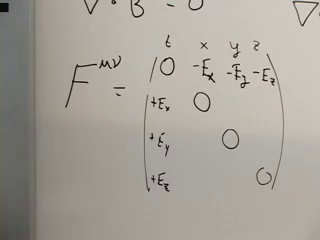
\includegraphics[width=0.58\textwidth]{lecture_58_figure_03.png}
\caption{Le tenseur électromagnétique complet, avec ses composantes électrique et magnétique.}
\lectureframe{00:32:05}
\end{figure}

L’importance de \(F^{\mu\nu}\) ne tient pas seulement au fait que six composantes du champ tiennent dans une même matrice. Sous une transformation de Lorentz, il se transforme comme un tenseur de rang deux. Les champs électrique et magnétique mesurés par des observateurs différents se mélangent donc exactement comme il le faut pour que l’ensemble se transforme de manière cohérente.

Il existe un second tenseur antisymétrique, le tenseur dual du champ \(\widetilde F^{\mu\nu}\). Avec la convention adoptée ici, on l’obtient à partir de l’équation~\eqref{eq:l0203-field-tensor} en effectuant le remplacement
\begin{equation}
\mathbf E\longmapsto-\mathbf B,
\qquad
\mathbf B\longmapsto\mathbf E.
\label{eq:dual-replacement}
\end{equation}
On obtient ainsi
\begin{equation}
\widetilde F^{\mu\nu}=
\begin{pmatrix}
0    & B_x  & B_y  & B_z\\
-B_x & 0    & -E_z & E_y\\
-B_y & E_z  & 0    & -E_x\\
-B_z & -E_y & E_x  & 0
\end{pmatrix}.
\label{eq:dual-tensor}
\end{equation}
Le signe dans l’équation~\eqref{eq:dual-replacement} est important. Pendant le cours, l’échange est d’abord énoncé verbalement ; on repère ensuite l’incohérence de signe et on la corrige avant de compléter la matrice.

\begin{figure}[H]
\centering
\includegraphics[width=0.58\textwidth]{lecture_58_figure_07.png}
\caption{Construction du tenseur dual par échange des composantes électrique et magnétique, avec le signe nécessaire.}
\lectureframe{00:35:45}
\end{figure}

\section{Les équations covariantes dans le vide}

Chaque équation de Maxwell contient une dérivée. La contraction d’un indice de dérivée avec un tenseur de rang deux laisse un indice libre ; les formes covariantes naturelles sont donc
\begin{align}
\partial_\mu F^{\mu\nu}&=0,
\label{eq:maxwell-covariant-vac}\\
\partial_\mu\widetilde F^{\mu\nu}&=0.
\label{eq:maxwell-dual-vac}
\end{align}
Pour chaque valeur fixée de \(\nu\), l’équation~\eqref{eq:maxwell-covariant-vac} constitue une équation. Comme \(\nu\) peut prendre les valeurs \(t,x,y,z\), elle regroupe quatre équations scalaires. L’équation~\eqref{eq:maxwell-dual-vac} en regroupe quatre autres. Cela correspond aux deux équations vectorielles faisant intervenir le rotationnel et aux deux équations scalaires de divergence de la liste initiale.

Une notation compacte n’est utile que si elle reproduit les équations familières. Prenons \(\nu=z\) :
\begin{align}
\partial_\mu F^{\mu z}
&=\partial_tF^{tz}
  +\partial_xF^{xz}
  +\partial_yF^{yz}
  +\partial_zF^{zz}\\
&=-\partial_tE_z+\partial_xB_y-\partial_yB_x\\
&=-\partial_tE_z+
  \bigl(\boldsymbol\nabla\times\mathbf B\bigr)_z.
\end{align}
Le terme \(F^{zz}\) s’annule par antisymétrie. En égalant le résultat à zéro, on obtient la composante \(z\) de
\begin{equation}
\boldsymbol\nabla\times\mathbf B=\partial_t\mathbf E.
\end{equation}
Les composantes \(x\) et \(y\) s’obtiennent par permutation cyclique des indices.

\begin{figure}[H]
\centering
\includegraphics[width=0.76\textwidth]{lecture_58_figure_08.png}
\caption{Développement en composantes de l’équation de champ covariante ; l’élément diagonal du tenseur s’annule et les termes restants reconstituent les équations de Maxwell.}
\lectureframe{00:43:30}
\end{figure}

Considérons maintenant la composante temporelle :
\begin{align}
\partial_\mu F^{\mu t}
&=\partial_tF^{tt}
  +\partial_xF^{xt}
  +\partial_yF^{yt}
  +\partial_zF^{zt}\\
&=\partial_xE_x+\partial_yE_y+\partial_zE_z\\
&=\boldsymbol\nabla\cdot\mathbf E.
\end{align}
On obtient donc l’équation~\eqref{eq:gauss-e-vac}. Les mêmes vérifications appliquées au tenseur dual donnent
\(\boldsymbol\nabla\cdot\mathbf B=0\) ainsi que
\(\boldsymbol\nabla\times\mathbf E=-\partial_t\mathbf B\).

Les équations compactes sont maintenant établies, et non simplement conjecturées. La structure de leurs indices libres en fait des équations à quatre composantes ; une transformation de Lorentz modifie donc leurs composantes, mais pas leur forme. C’est en ce sens précis que les équations de Maxwell dans le vide sont les mêmes dans tous les référentiels inertiels.

\section{Des équations du premier ordre aux ondes}

Les équations de Maxwell ne contiennent que des dérivées du premier ordre, tandis qu’une équation d’onde fait intervenir des dérivées secondes. Cette différence apparente s’explique par le couplage entre deux champs dans la théorie de Maxwell. En combinant deux équations du premier ordre pour \(\mathbf E\) et \(\mathbf B\), on peut obtenir une équation du second ordre pour chacun des champs pris séparément.

Dérivons l’équation~\eqref{eq:ampere-vac} par rapport au temps :
\begin{equation}
\partial_t^2\mathbf E
=\boldsymbol\nabla\times\partial_t\mathbf B.
\end{equation}
La loi de Faraday fournit la dérivée temporelle de \(\mathbf B\) :
\begin{equation}
\partial_t\mathbf B=-\boldsymbol\nabla\times\mathbf E,
\end{equation}
et donc
\begin{equation}
\partial_t^2\mathbf E
=-\boldsymbol\nabla\times
  \bigl(\boldsymbol\nabla\times\mathbf E\bigr).
\label{eq:double-curl}
\end{equation}

Le calcul au tableau développe une composante plutôt que de faire appel à une identité apprise par cœur. Pour la composante \(x\),
\begin{align}
\bigl[\boldsymbol\nabla\times
(\boldsymbol\nabla\times\mathbf E)\bigr]_x
&=\partial_y(\boldsymbol\nabla\times\mathbf E)_z
 -\partial_z(\boldsymbol\nabla\times\mathbf E)_y\\
&=\partial_y(\partial_xE_y-\partial_yE_x)\\
&\quad-\partial_z(\partial_zE_x-\partial_xE_z)\\
&=\partial_x(\partial_yE_y+\partial_zE_z)
 -\partial_y^2E_x\\
&\quad-\partial_z^2E_x.
\end{align}
Ajoutons et retranchons \(\partial_x^2E_x\) afin de faire apparaître la divergence :
\begin{align}
\bigl[\boldsymbol\nabla\times
(\boldsymbol\nabla\times\mathbf E)\bigr]_x
&=\partial_x(\boldsymbol\nabla\cdot\mathbf E)
 -\nabla^2E_x.
\label{eq:double-curl-x}
\end{align}
Dans le vide, \(\boldsymbol\nabla\cdot\mathbf E=0\). En combinant les équations~\eqref{eq:double-curl} et \eqref{eq:double-curl-x}, on obtient
\begin{equation}
\left(\partial_t^2-\nabla^2\right)E_x=0.
\label{eq:ex-wave}
\end{equation}

\begin{figure}[H]
\centering
\includegraphics[width=0.72\textwidth]{lecture_58_figure_09.png}
\caption{Le calcul en composantes aboutit à l’équation d’onde pour \(E_x\).}
\lectureframe{00:57:10}
\end{figure}

Le même calcul s’applique à \(E_y\) et \(E_z\), et une élimination analogue donne
\begin{equation}
\left(\partial_t^2-\nabla^2\right)\mathbf B=0.
\end{equation}
Les champs électrique et magnétique peuvent donc se propager dans le vide sous forme d’ondes. Dans les unités utilisées ici, leur vitesse vaut un ; en rétablissant les unités usuelles, elle vaut \(c\).

\section{Onde plane et polarisation}

Construisons une onde simple qui se propage dans la direction positive de \(z\) :
\begin{equation}
\mathbf E(z,t)
=\widehat{\mathbf x}\,E_0
  \cos\!\bigl(k(z-t)\bigr).
\label{eq:plane-e}
\end{equation}
Son profil se propage le long de \(z\) sans changer de forme. Le champ électrique étant orienté selon l’axe \(x\), l’onde est polarisée linéairement dans la direction \(x\). Nous avons choisi \(E_y=0\) uniquement pour simplifier l’exemple ; on pourrait y ajouter une seconde polarisation transverse.

La composante longitudinale n’est pas tout aussi libre. Puisque l’onde ne dépend que de \(z\) et de \(t\),
\begin{equation}
\boldsymbol\nabla\cdot\mathbf E
=\partial_zE_z=0.
\end{equation}
Ainsi, \(E_z\) peut être constant, mais ne peut pas contenir le profil ondulatoire variable. On peut ajouter ou supprimer indépendamment un champ uniforme de fond ; il ne fait pas partie du rayonnement qui se propage. L’onde elle-même est transverse :
\begin{equation}
\mathbf E_{\mathrm{wave}}\cdot\widehat{\mathbf z}=0.
\end{equation}

La loi de Faraday détermine le champ magnétique. Pour l’équation~\eqref{eq:plane-e}, la seule composante non nulle de \(\boldsymbol\nabla\times\mathbf E\) est la composante \(y\) :
\begin{equation}
(\boldsymbol\nabla\times\mathbf E)_y=\partial_zE_x.
\end{equation}
Par conséquent, \(\partial_t\mathbf B\) est orienté selon \(y\), et un choix compatible est
\begin{equation}
\mathbf B(z,t)
=\widehat{\mathbf y}\,E_0
  \cos\!\bigl(k(z-t)\bigr).
\label{eq:plane-b}
\end{equation}
Dans ces unités, les amplitudes électrique et magnétique sont égales. Leur orientation vérifie
\begin{equation}
\mathbf E\perp\mathbf B,
\qquad
\mathbf E\perp\widehat{\mathbf z},
\qquad
\mathbf B\perp\widehat{\mathbf z},
\qquad
\mathbf E\times\mathbf B\parallel\widehat{\mathbf z}.
\end{equation}

\begin{figure}[H]
\centering
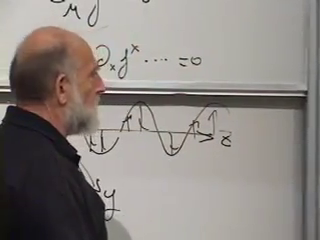
\includegraphics[width=0.70\textwidth]{lecture_58_figure_05.png}
\caption{Schéma complet au tableau d’une onde électromagnétique transverse : les oscillations électrique et magnétique sont perpendiculaires l’une à l’autre et à la direction de propagation.}
\lectureframe{01:05:25}
\end{figure}

\begin{figure}[H]
\centering
\scalebox{0.90}{%
\begin{tikzpicture}[x=1cm,y=1cm,>=Latex]
  \draw[->,thick] (0,0) -- (8.2,0) node[right] {$z$};
  \draw[->,thick] (0,-1.6) -- (0,1.7) node[above] {$x$};
  \draw[->,thick] (0,0) -- (-1.15,-0.8) node[below left] {$y$};
  \draw[blue!70!black,thick,domain=0:7.5,samples=120]
    plot (\x,{0.95*sin(90*\x)});
  \foreach \z/\s in {0.8/1,2.8/-1,4.8/1,6.8/-1}{
    \draw[->,green!45!black,thick]
      (\z,0) -- ++({-0.55*\s},{-0.38*\s});
  }
  \node[blue!70!black] at (6.9,1.25) {$\mathbf E$};
  \node[green!45!black] at (5.2,-1.05) {$\mathbf B$};
  \draw[->,very thick] (6.2,1.55) -- (7.7,1.55)
    node[midway,above] {propagation};
\end{tikzpicture}
}
\caption{Les champs \(\mathbf E\) et \(\mathbf B\) sont perpendiculaires l’un à l’autre et à la direction de propagation.}
\end{figure}

C’est le caractère de la lumière et de tout rayonnement électromagnétique dans le vide. Comme les équations qui produisent l’onde sont covariantes de Lorentz, un autre observateur inertiel décrit lui aussi une onde électromagnétique se déplaçant à \(c\), avec des champs électrique et magnétique transverses.

\section{Densité de charge et densité de courant}

Réintroduisons maintenant les sources que nous avions provisoirement mises de côté. Lorsqu’une région contient de nombreuses particules chargées, il est utile de les décrire à une échelle macroscopique par une densité de charge continue :
\begin{equation}
\rho(\mathbf x,t)=\frac{dQ}{dV}.
\end{equation}
Cette approximation revient à traiter l’eau comme un fluide continu, bien qu’elle soit constituée de molécules. Les charges positives et négatives contribuent avec des signes opposés ; \(\rho\) est donc la charge nette par unité de volume.

La charge contenue dans une région donnée \(V\) est
\begin{equation}
Q_V(t)=\int_V\rho(\mathbf x,t)\,dV.
\label{eq:charge-volume}
\end{equation}
La densité peut varier dans l’espace et au cours du temps. Une accumulation de charges peut quitter un point, ce qui modifie la densité locale à cet endroit. Cette variation ne peut toutefois pas être arbitraire. La nature conserve la charge électrique.

La seule conservation globale serait trop peu contraignante. Elle permettrait à la charge de disparaître de la Terre et de réapparaître sur Mars au même instant, tout en laissant la charge totale inchangée. L’énoncé plus fort est local : la charge ne peut quitter un endroit pour en atteindre un autre qu’en circulant dans l’espace intermédiaire.

Pour décrire cet écoulement, considérons un élément de surface orienté infinitésimal :
\begin{equation}
d\boldsymbol\sigma=\widehat{\mathbf n}\,d\sigma.
\end{equation}
Sa norme est l’aire, et sa direction est normale à la surface. La densité de courant \(\mathbf J\) est définie de sorte que la charge traversant cet élément par unité de temps soit
\begin{equation}
\frac{dQ}{dt}=\mathbf J\cdot d\boldsymbol\sigma.
\label{eq:current-flux-element}
\end{equation}
La norme de \(\mathbf J\) correspond à une charge par unité d’aire et de temps, et sa direction indique le sens d’écoulement des charges positives.

\begin{figure}[H]
\centering
\includegraphics[width=0.64\textwidth]{lecture_58_figure_10.png}
\caption{Élément de surface orienté et facteur de flux \(d\boldsymbol\sigma\cdot\mathbf J\).}
\lectureframe{01:18:15}
\end{figure}

Le produit scalaire sélectionne la composante normale à la surface. Un courant tangent à la surface ne la traverse ni d’un côté ni de l’autre et contribue donc pour zéro. Pour une norme donnée, le courant parallèle à la normale produit le flux maximal. Le courant dans un fil n’est qu’un cas particulier ; \(\mathbf J\) peut aussi décrire un écoulement de charge à travers une feuille ou dans tout un espace tridimensionnel.

\section{Conservation locale et équation de continuité}

Fixons une région \(V\) de l’espace et orientons vers l’extérieur chaque élément de sa frontière fermée \(\partial V\). Si le courant net sortant est positif, la charge contenue dans la région diminue :
\begin{equation}
\frac{dQ_V}{dt}
=-\oint_{\partial V}\mathbf J\cdot d\boldsymbol\sigma.
\label{eq:integral-conservation}
\end{equation}
Le signe moins traduit une réalité physique, il n’est pas dû à une convention : un flux positif sortant retire de la charge positive de la région. En utilisant l’équation~\eqref{eq:charge-volume},
\begin{equation}
\int_V\partial_t\rho\,dV
=-\oint_{\partial V}\mathbf J\cdot d\boldsymbol\sigma.
\label{eq:integral-continuity-one}
\end{equation}

\begin{figure}[H]
\centering
\includegraphics[width=0.72\textwidth]{lecture_58_figure_11.png}
\caption{Loi de conservation dans une région fixe, après conversion du flux à travers la surface en une intégrale de volume.}
\lectureframe{01:29:00}
\end{figure}

Le théorème de Gauss, aussi appelé théorème de la divergence, relie le flux à travers une surface fermée à la divergence à l’intérieur de celle-ci :
\begin{equation}
\oint_{\partial V}\mathbf A\cdot d\boldsymbol\sigma
=\int_V\boldsymbol\nabla\cdot\mathbf A\,dV.
\label{eq:divergence-theorem}
\end{equation}
On peut imaginer des conduits cachés qui injectent de l’eau en différents points à l’intérieur d’un récipient. La divergence mesure le débit local auquel l’eau sort des extrémités des conduits ; l’intégrale de surface mesure la quantité totale d’eau qui quitte le récipient. Toute l’eau qui s’écoule vers l’extérieur depuis l’intérieur doit finir par traverser la frontière.

En appliquant l’équation~\eqref{eq:divergence-theorem} à \(\mathbf J\), on obtient
\begin{equation}
\int_V
\left(\partial_t\rho+\boldsymbol\nabla\cdot\mathbf J\right)dV=0.
\end{equation}
Cette relation vaut pour toute région possible \(V\). L’intégrande doit donc s’annuler en chaque point :
\begin{equation}
\boxed{\partial_t\rho+\boldsymbol\nabla\cdot\mathbf J=0.}
\label{eq:continuity-three}
\end{equation}

\begin{figure}[H]
\centering
\includegraphics[width=0.72\textwidth]{lecture_58_figure_12.png}
\caption{Équation locale de continuité écrite composante par composante.}
\lectureframe{01:29:50}
\end{figure}

L’équation~\eqref{eq:continuity-three} exprime exactement ce qu’exige la conservation locale. Si la densité de charge diminue en un point ou dans une petite région, le courant doit diverger vers l’extérieur. Si le courant converge vers l’intérieur, la densité de charge augmente.

La densité et le courant forment naturellement le quadri-courant
\begin{equation}
J^\mu=(\rho,J_x,J_y,J_z)
\label{eq:four-current}
\end{equation}
dans les unités \(c=1\). L’équation de continuité prend la forme de l’équation scalaire de Lorentz
\begin{equation}
\partial_\mu J^\mu=0.
\label{eq:continuity-four}
\end{equation}
Le flux associé à une distribution relativiste doit se transformer comme un quadrivecteur, tout comme la quadrivitesse d’une particule. L’équation~\eqref{eq:continuity-four} garantit la conservation locale de la charge dans tous les référentiels inertiels.

\section{Les équations de Maxwell avec sources}

En réintroduisant la charge et le courant, on obtient
\begin{align}
\boldsymbol\nabla\cdot\mathbf E&=\rho,
\label{eq:gauss-e-source}\\
\boldsymbol\nabla\cdot\mathbf B&=0,\\
\boldsymbol\nabla\times\mathbf E&=-\partial_t\mathbf B,\\
\boldsymbol\nabla\times\mathbf B&=\partial_t\mathbf E+\mathbf J.
\label{eq:ampere-source}
\end{align}
Les équations faisant intervenir les sources électriques se condensent en
\begin{equation}
\boxed{\partial_\mu F^{\mu\nu}=J^\nu,}
\label{eq:maxwell-source-covariant}
\end{equation}
tandis que la paire magnétique sans source reste
\begin{equation}
\boxed{\partial_\mu\widetilde F^{\mu\nu}=0.}
\label{eq:maxwell-dual-source}
\end{equation}

\begin{figure}[H]
\centering
\includegraphics[width=0.78\textwidth]{lecture_58_figure_13.png}
\caption{Les équations de Maxwell avec sources, accompagnées de leur forme covariante \(\partial_\mu F^{\mu\nu}=J^\nu\).}
\lectureframe{01:34:00}
\end{figure}

La composante temporelle de l’équation~\eqref{eq:maxwell-source-covariant} s’écrit
\begin{equation}
\partial_\mu F^{\mu t}=J^t=\rho,
\end{equation}
et le calcul en composantes déjà effectué transforme son membre de gauche en
\(\boldsymbol\nabla\cdot\mathbf E\). Les trois composantes spatiales redonnent
\(\boldsymbol\nabla\times\mathbf B=\partial_t\mathbf E+\mathbf J\).

On dispose également d’une vérification utile de cohérence. Appliquons \(\partial_\nu\) à l’équation~\eqref{eq:maxwell-source-covariant} :
\begin{equation}
\partial_\nu J^\nu
=\partial_\nu\partial_\mu F^{\mu\nu}=0,
\end{equation}
car les deux dérivées sont symétriques sous l’échange \(\mu\leftrightarrow\nu\), tandis que \(F^{\mu\nu}\) est antisymétrique.\editorialnote{Cette courte vérification de cohérence découle de l’équation covariante et montre explicitement pourquoi les équations de Maxwell avec sources respectent automatiquement l’équation de continuité.}

La structure réciproque est maintenant complète. La loi de force tensorielle
\(f^\mu=qF^\mu{}_\nu u^\nu\)
décrit l’action des champs sur les charges, et l’équation~\eqref{eq:maxwell-source-covariant} décrit comment les charges et les courants produisent les champs. Ces deux relations sont des équations tensorielles. Dans le vide, les mêmes équations de champ conduisent à des ondes transverses se propageant à \(c\). La covariance de Lorentz et l’équation d’onde électromagnétique se rejoignent donc au point qui a motivé toute cette construction : tous les observateurs inertiels obtiennent les mêmes lois de l’électromagnétisme et la même vitesse de la lumière.
